\section{System Design}
\label{sec:system-design}

\subsection{System Architecture}
\label{subsec:system-architecture}

\subsubsection*{Engine Design}

The project's core engine design, as stated before, will use an ECS framework that registers and
determines components and system dependencies at compile-time.
The declaration of a single ECS instance that registers all components and systems would result in
wasteful usage of memory and projected performance decreases due to the large variety of components involved.
As such, we have opted to use multiple smaller ECS instances that each take control of a smaller part of the game.
We refer to these smaller ECS instances, alongside the data necessary to register related components and systems,
as well as compute and store initial data into those instances, as scenes.
Communications between scenes, such as the data transfer when creating a new scene, are facilitated through
a SceneManager, which will also execute the registered systems during the main game loop.

\vspace{0.5cm}

\noindent
\begin{minipage}{\columnwidth}
    \centering
    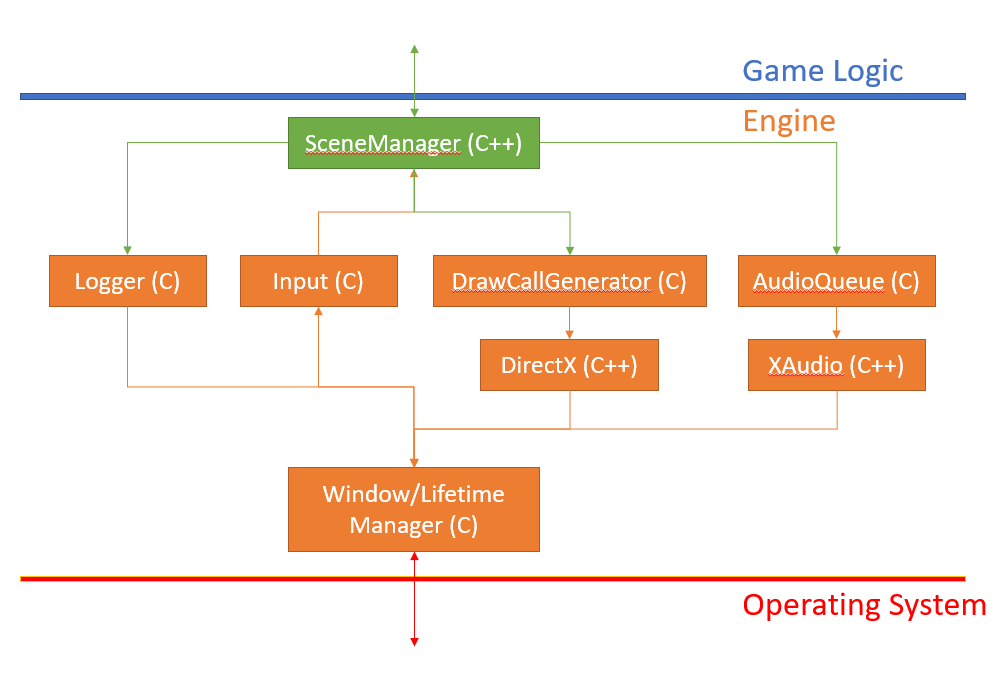
\includegraphics[width=\columnwidth, keepaspectratio]{images/engine}
    \captionof{figure}{A diagram showing data flow of the engine prototype}
    \label{fig:engine}
\end{minipage}

\vspace{0.5cm}

\noindent Figure~\ref{fig:engine} shows the outline of the engine.
The SceneManager takes ownership and executes user-level systems during runtime by receiving inputs from the operating system,
passing logs, audio, and render-object references to different specialized components.
Those components will then pass information to the operating system to pass information to the device outputs as appropriate.
For modularity, the communications are passed through the Windows/Lifetime Manager, which acts as an adapter for the operating system.
\\\\
For the actual implementation of these compile-time optimizations, we take advantage of C++'s concept of templates.
By using component and system data types as template parameters, we can use template specialization to let
the compiler generate code specific to our use case.
Since each system is a function, this also means we get usage of functions without relying on indirect calls,
which is a common pain point in engine design.
\\\\
The benefits of template specialization can be seen with a key part of the ECS instance, the resource manager.
The resource manager manages entities along with any components attached to those entities, together referred to as resources.
The resource manager takes a size integer and any number of structures as template parameters and treats those
structures as registered components in this instance.
It will create a resource pool of each registered component with the specified size when constructed, each of
which will reserve their own memory depending on the component's size and the pool size.
By accessing these components through template specialization, code is generated such that the abstraction layers
are removed from the code when compiled.
\\\\
While systems are being run, entities with select component archetypes are iterated upon.
If components are added or removed during iteration, this may invalidate references or otherwise cause unpredictable behavior.
To avoid such hazards, a structure must be created with the purpose to defer all attempts to add or remove components
and to apply such changes after all systems complete execution.
Borrowing the term from operating systems, we refer to this structure with elevated permissions to modify resources
as the syscall.
The syscall must know the components registered to its coupled resource manager so that it can add the appropriate
components.
When systems want to add or remove components from an entity, they make the request to the ECS instance, which
will schedule the changes in its internal syscall.
\\\\
Systems operate upon entities based on whether they fulfill certain component requirements.
For complex systems, the requirements can be rather complex, and entities may be retrieved multiple times
under different requirements.
Some implementations have the ECS instance be provided as a function argument to each system so that entities
can be retrieved directly from internal resources via templated retrieval functions.
We decided, instead, that systems define query data structures as function arguments, which describes the components
that entity references stored within are guaranteed to possess.
When the system is run, the ECS instance will internally fulfill each query requirement by fetching and filtering
from the resource manager before passing them to the system.
This way, the system's implementation does not concern itself with fetching data from the ECS instance.

\subsubsection*{Game Design}

The project's core game design will involve combining rhythm games and bullet hell games into a hybrid game
structured around distinct but smoothly transitioning phases.
This requires a seamless transition between the two to create a revolutionary take on hybrid games.
Considering that both of the games hugely relied on great optimization, as with a little disruption,
it can cause a fatal mistake for the player inciting frustration, the design of the game must be made cautiously.
\\\\
\noindent The bullet hell section is mostly composed of large numbers of bullets and particles,
while great performance is still required to retain the player’s fluidity of movement.
ECS architecture is highly favored as opposed to object-oriented programming since the
large number of entities can be handled more efficiently.
Entities of the system are composed of player, bullets, boss, enemies, background, and effects
using shared components such as position, velocity, sprite, and shader.
Each system must be executed every frame to handle entity movement,
collision check, and player input, allowing it to handle every bullet in a frame efficiently.

\vspace{0.5cm}

\noindent
\begin{minipage}{\columnwidth}
    \centering
    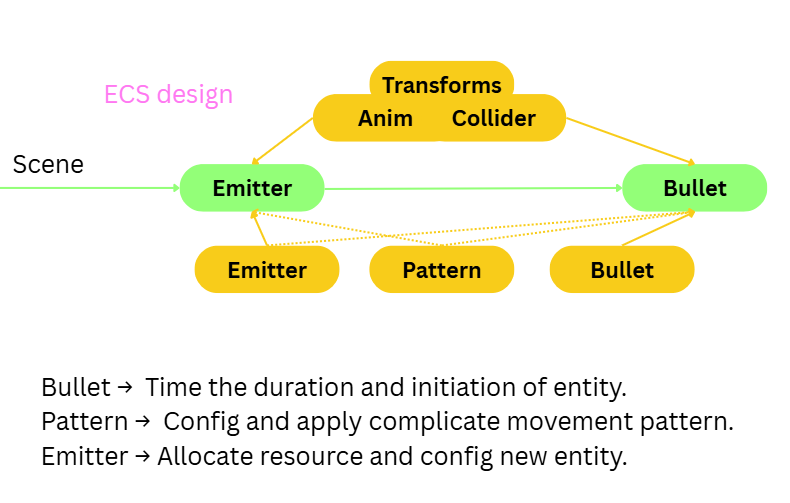
\includegraphics[width=\columnwidth, keepaspectratio]{images/designbullet}
    \captionof{figure}{Preliminary system design for the bullet hell gameplay section}
    \label{fig:designbullet}
\end{minipage}

\vspace{0.5cm}

\noindent Figure~\ref{fig:designbullet} shows the current system design for bullet hell gameplay.
A bullet loader entity is initialized during the initiation process of the scene alongside all bullet data used within the scene.
The bullet loader system then spawn bullets from the data stored in its component at the configured frame timing.
Each spawned bullet data entry contains a stage bullet ID used to retrieve additional information from the stage bullet registry.
This registry also references a graphic ID to query even more data from the bullet graphic registry.
After all required data is gathered, the bullet entity is spawned with its components configured from the gathered data.
\\\\
The core mechanics are that, for each frame, the input was processed to control the player system.
Meanwhile, the collision system will check each ongoing colliding entity by computing if each entity with a collider component
is colliding with another entity.
Then, the corresponding function will be triggered to apply change to the state such as the player taking damage.
Moreover, the movement system computes the next frame position to render, and the animation system will update the animation frame of the sprite to be rendered.
\\\\
On the other hand, rhythm games require precise timing to catch the notes at the right time,
so very few optimization issues can be tolerated as a result.
However, ECS architecture is powerful enough to handle all the requirements
such as a large quantity of notes and an accurate time tracking device centralized by the clock system.

\vspace{0.5cm}

\noindent
\begin{minipage}{\columnwidth}
    \centering
    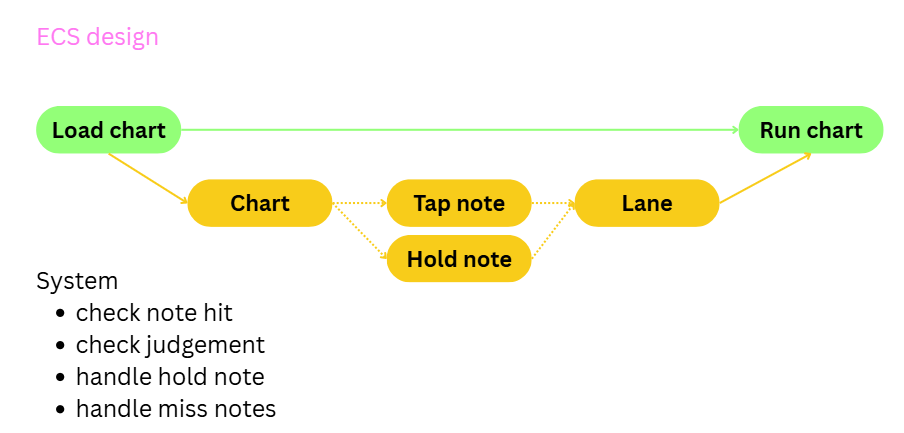
\includegraphics[width=\columnwidth, keepaspectratio]{images/designrhythm}
    \captionof{figure}{Preliminary system design of the rhythm game gameplay section}
    \label{fig:designrhythm}
\end{minipage}

\vspace{0.5cm}

\noindent Figure~\ref{fig:designrhythm} shows the current system design for rhythm game section.
When the game scene is initiated, a chart entity containing the note data is retrieved.
Each note data entry contains a note type, timing, and lane information.
Then, the note loading system will create note entities with each one being in one of the four lanes.
Unlike the bullet hell section, the notes can be loaded all at once since its initial position is determined by the lane.
After all the notes are created, the scene will be running and the systems will be executed every frame to update the note position and check for player input.
\\\\
The core mechanic revolves around spawning the notes at the right time and calculating the position of the sprite as it moves.
However, the real logic of the note is being computed by its own system depending on its type, such as tap note and hold note.
Once the note reaches its timing range, the system will check the timing of the player's input and
display the corresponding accuracy known as judgment.
\\\\
Transitioning between both types of gameplay proves to be a great challenge design-wise, as it has to be
smooth and seamless enough to not disrupt the precision-hungry gameplay of both games.
To ensure a smooth gameplay experience, only one game scene is rendered to minimize time to transition
as the whole scene will be loaded and initiated only once from the start.
If the transition is happening, the gameplay should be frozen and any progress should not be considered during the process,
allowing the player to get ready to adjust their gameplay smoothly.
Also, the transition's animation has to telegraph the player clearly to make them aware that the gameplay is going to be changed
by including a countdown to inform the duration of the transition.
% Lastly, the screen changing the gameplay rendered has to be creative and visually appealing to not make the transition jarring or out of place.
% % To achieve this, a line animation system is used to express animation of the transition, and the game transition system
% % will be triggered if the state has been changed.
% One of the proposed transitions is a line animation that starts from the center of the screen and expands until it covers the whole screen.
% Following this, the new gameplay is rendered for a section of the screen expanding until full.
\\\\
The biggest concern of the game logic is the control of the rhythm game's charts and bullet hell's patterns
needing to not be exhaustingly difficult to control, as both games require vast amounts of complicated pattern and timing design.
A solution proposed was to create our own scripting language and a corresponding compiler.
This allows game developers to create levels in a file format that is easy to read and write,
while the compiler can convert it into a format that can be processed by the game engine.
Practicing these techniques makes designing and implementing charts and patterns easier,
allowing more complex and challenging designs and features.
\\\\
% To complete a game, a narrative device should be implemented to make the game more immersive and enjoyable;
% the proposed gameplay would be a 2D side-scrolling style that allows players to choose a level and progress the story of the game.
% Additionally, explorations are added to the game such as interacting with interactable entities such as NPC, or objects,
% getting new in-game items, and accessing new areas.
% Such requirements must be implemented with an entirely separate game logic.
% Interactable and solid collision components are needed to be implemented along with the new system,
% for example, a new movement system, interact system, and area load system.
% \\\\
Lastly, using ECS, UI entities are being rendered concurrently in a higher priority by default.
The entities will have a position, text, sprite, and animation components and are created orderly using functions for each set of UIs.
For audios in the game, including sound effects and music, each is assigned to its own entity with a tag or trigger to be played on an instance sound system.
\\\\
In the future, we plan to add a narrative device to make the game more immersive and enjoyable;
the proposed gameplay would be a 2D side-scrolling style that allows players to choose a level and progress the story,
with the ability to interact with NPCs and objects, and access new areas.

\subsection{Components}
\label{subsec:components}

The system is a self-contained application, but interfacing with a keyboard and mouse is required for its operation.
DirectX 11 is used for the rendering of the game with the use of a custom rendering pipeline implementation.
User input is collected through the Windows API\@.

\subsection{Design Considerations}
\label{subsec:design-considerations}

% Performance, scalability, usability, sustainability, environment
We formed the design with considerations of usability at the forefront.
The interface was to allow user-level system design to be as close to natural C++ functional design as possible,
while still retaining the power of ECS systems.
We also ensured the design allowed for aggressive compiler optimization and inlining by avoiding virtual function calls,
abstractions with hidden costs or overhead, and pointer arithmetic whose behaviors are challenging to predict.
The architecture was highly modular with little coupling to allow for incremental additions to the engine during the
implementation process and in future works.

\subsection{Proposed vs. Final Design}
\label{subsec:proposed-vs-final}

The proposed engine design did not undergo major changes in the implementation process.
As the design is modular, as the engine's execution is optimized, modules that serve the same purpose were being swapped out
with more efficient ones that serve the same function.
\\\\
Meanwhile, some gameplay systems were adjusted to increase the maintainability of the code in future development.
The bullet hell system architecture was mostly restructured using bullet registry to handle the large variety of bullet
patterns and graphics, allowing the bullet loader system to be more generalized.
The rhythm game system was also refactored to accommodate different note types and hit detection logic, allowing for more flexible
and implementable features.

